\documentclass{article}
\usepackage[utf8]{inputenc}
\usepackage{graphicx}
\usepackage[pdftex]{hyperref}



\title{Laboratório 03}
\author{Amanda Goulart - 133569}
\date{Outubro 2020}

\begin{document}



\section{Problema}
Utilizando o laboratório 03 como base, substitua o valor de B por uma multiplicação entre dois
números C e D.
\\
C é um valor da soma de dois dados, conforme utilizado no laboratório 02.
D deve ser um valor entre as seguintes possibilidades: 2, 3, 4, 5.
Assim, o circuito deve conter como entradas os bits correspondentes a dois dados (valor de C), um
seletor para quatro possibilidades entre os possíveis valores de D e o valor do caixa A de 8 bits.
\\
Todos
esses números são naturais. Também precisará de um seletor de operação soma ou subtração, como no
laboratório 03.
\\
Como saída, o circuito deve ter o valor final do caixa A +/- C * D mostrado em um conjunto de 3
displays de 7 segmentos da mesma maneira que no laboratório 03. Continue a usar os valores --- e 999
para quando o resultado da operação é negativo ou estourar o limite.
\\
Use também mais 3 displays de 7
segmentos para apresentar o valor inicial de A, dois displays para mostrar os valores dos dados sendo
um display por dado e um conjunto de 3 displays de para mostrar o resultado da multiplicação de C por
D.
\section{Solução}

\subsubsection{C}

Para o valor de C, utilizei a implementação do laboratório 02, mas só utilizando a parte de 1 jogador.
\\
\\
\\
\\
\\
\\
\\
\\
\begin{figure}[!h]
\centering
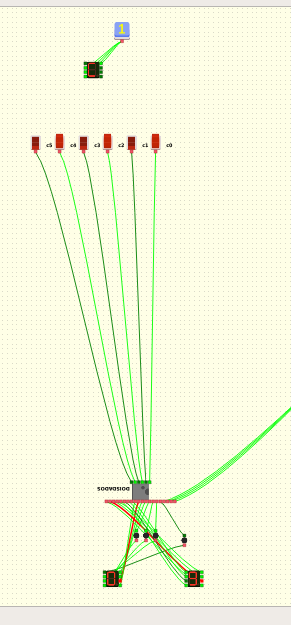
\includegraphics[width=5cm]{c.png}
\caption{Soma de dois dados}
\label{fig:CL_logo}
\end{figure}

\subsubsection{D}

Como o valor de D é 2 bits que valem o {2,3,4,5}, considerei os seguintes valores:

% ######## init table ########
\begin{table}[h]
 \centering
% distancia entre a linha e o texto
 {\renewcommand\arraystretch{1.25}
 \begin{tabular}{ l l l l l l }
  \cline{1-1}\cline{2-2}\cline{3-3}\cline{4-4}\cline{5-5}\cline{6-6}
    \multicolumn{1}{|c|}{x0} &
    \multicolumn{1}{c|}{x1} &
    \multicolumn{1}{c|}{y0} &
    \multicolumn{1}{c|}{y1} &
    \multicolumn{1}{c|}{y2} &
    \multicolumn{1}{c|}{D}
  \\
  \cline{1-1}\cline{2-2}\cline{3-3}\cline{4-4}\cline{5-5}\cline{6-6}
    \multicolumn{1}{|c|}{0} &
    \multicolumn{1}{c|}{0} &
    \multicolumn{1}{c|}{0} &
    \multicolumn{1}{c|}{1} &
    \multicolumn{1}{c|}{0} &
    \multicolumn{1}{c|}{2}
  \\
  \cline{1-1}\cline{2-2}\cline{3-3}\cline{4-4}\cline{5-5}\cline{6-6}
    \multicolumn{1}{|c|}{0} &
    \multicolumn{1}{c|}{1} &
    \multicolumn{1}{c|}{0} &
    \multicolumn{1}{c|}{1} &
    \multicolumn{1}{c|}{1} &
    \multicolumn{1}{c|}{3}
  \\
  \cline{1-1}\cline{2-2}\cline{3-3}\cline{4-4}\cline{5-5}\cline{6-6}
    \multicolumn{1}{|c|}{1} &
    \multicolumn{1}{c|}{0} &
    \multicolumn{1}{c|}{1} &
    \multicolumn{1}{c|}{0} &
    \multicolumn{1}{c|}{0} &
    \multicolumn{1}{c|}{4}
  \\
  \cline{1-1}\cline{2-2}\cline{3-3}\cline{4-4}\cline{5-5}\cline{6-6}
    \multicolumn{1}{|c|}{1} &
    \multicolumn{1}{c|}{1} &
    \multicolumn{1}{c|}{1} &
    \multicolumn{1}{c|}{0} &
    \multicolumn{1}{c|}{1} &
    \multicolumn{1}{c|}{5}
  \\
  \hline

 \end{tabular} }
\end{table}

Realizando o mapa de Karnaugh:

Para y0:
\\
\\
\\
\\
\\
\begin{figure}[!h]
\centering
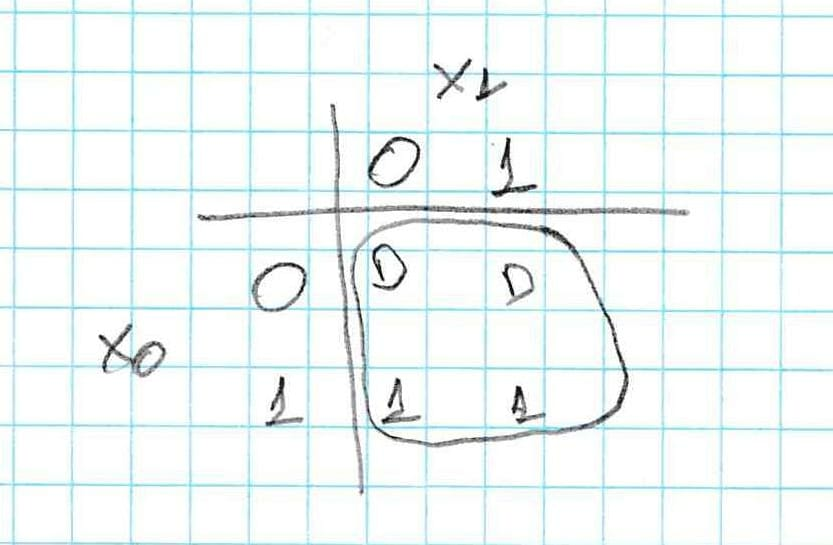
\includegraphics[width=5cm]{y0.jpeg}
\caption{Mapa de Karnaugh para y0}
\label{fig:CL_logo}
\end{figure}

Resultando em 1.

Para y1:

\begin{figure}[!h]
\centering
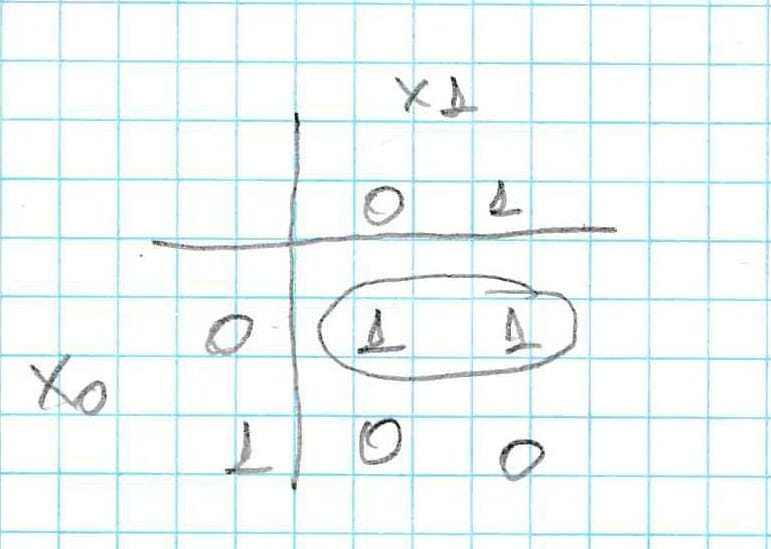
\includegraphics[width=5cm]{y1.jpeg}
\caption{Mapa de Karnaugh para y1}
\label{fig:CL_logo}
\end{figure}

Resultando em: \overline{x0}

Para y2:

\begin{figure}[!h]
\centering
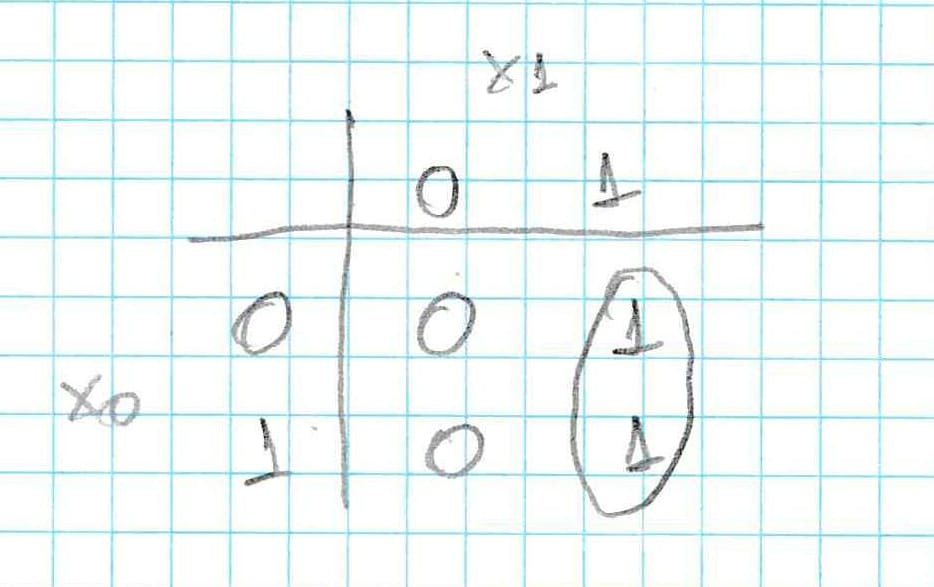
\includegraphics[width=5cm]{y2.jpeg}
\caption{Mapa de Karnaugh para y2}
\label{fig:CL_logo}
\end{figure}


Resultando em x1.


Com o circuito final:
\\
\\
\\
\\
\\
\\
\\
\begin{figure}[!h]
\centering
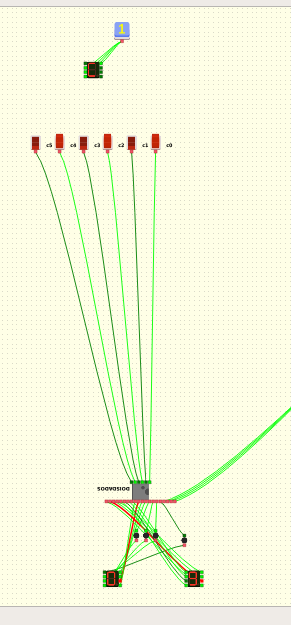
\includegraphics[width=5cm]{c.png}
\caption{Circuito para D}
\label{fig:CL_logo}
\end{figure}


\section{Multiplicação de C e D}

Para a multiplicação utilizei o circuito disponibilizado no slide.
Resultando no seguinte circuito:
\\

\\
\\
\\
\\
\\
\\

\begin{figure}[!h]
\centering
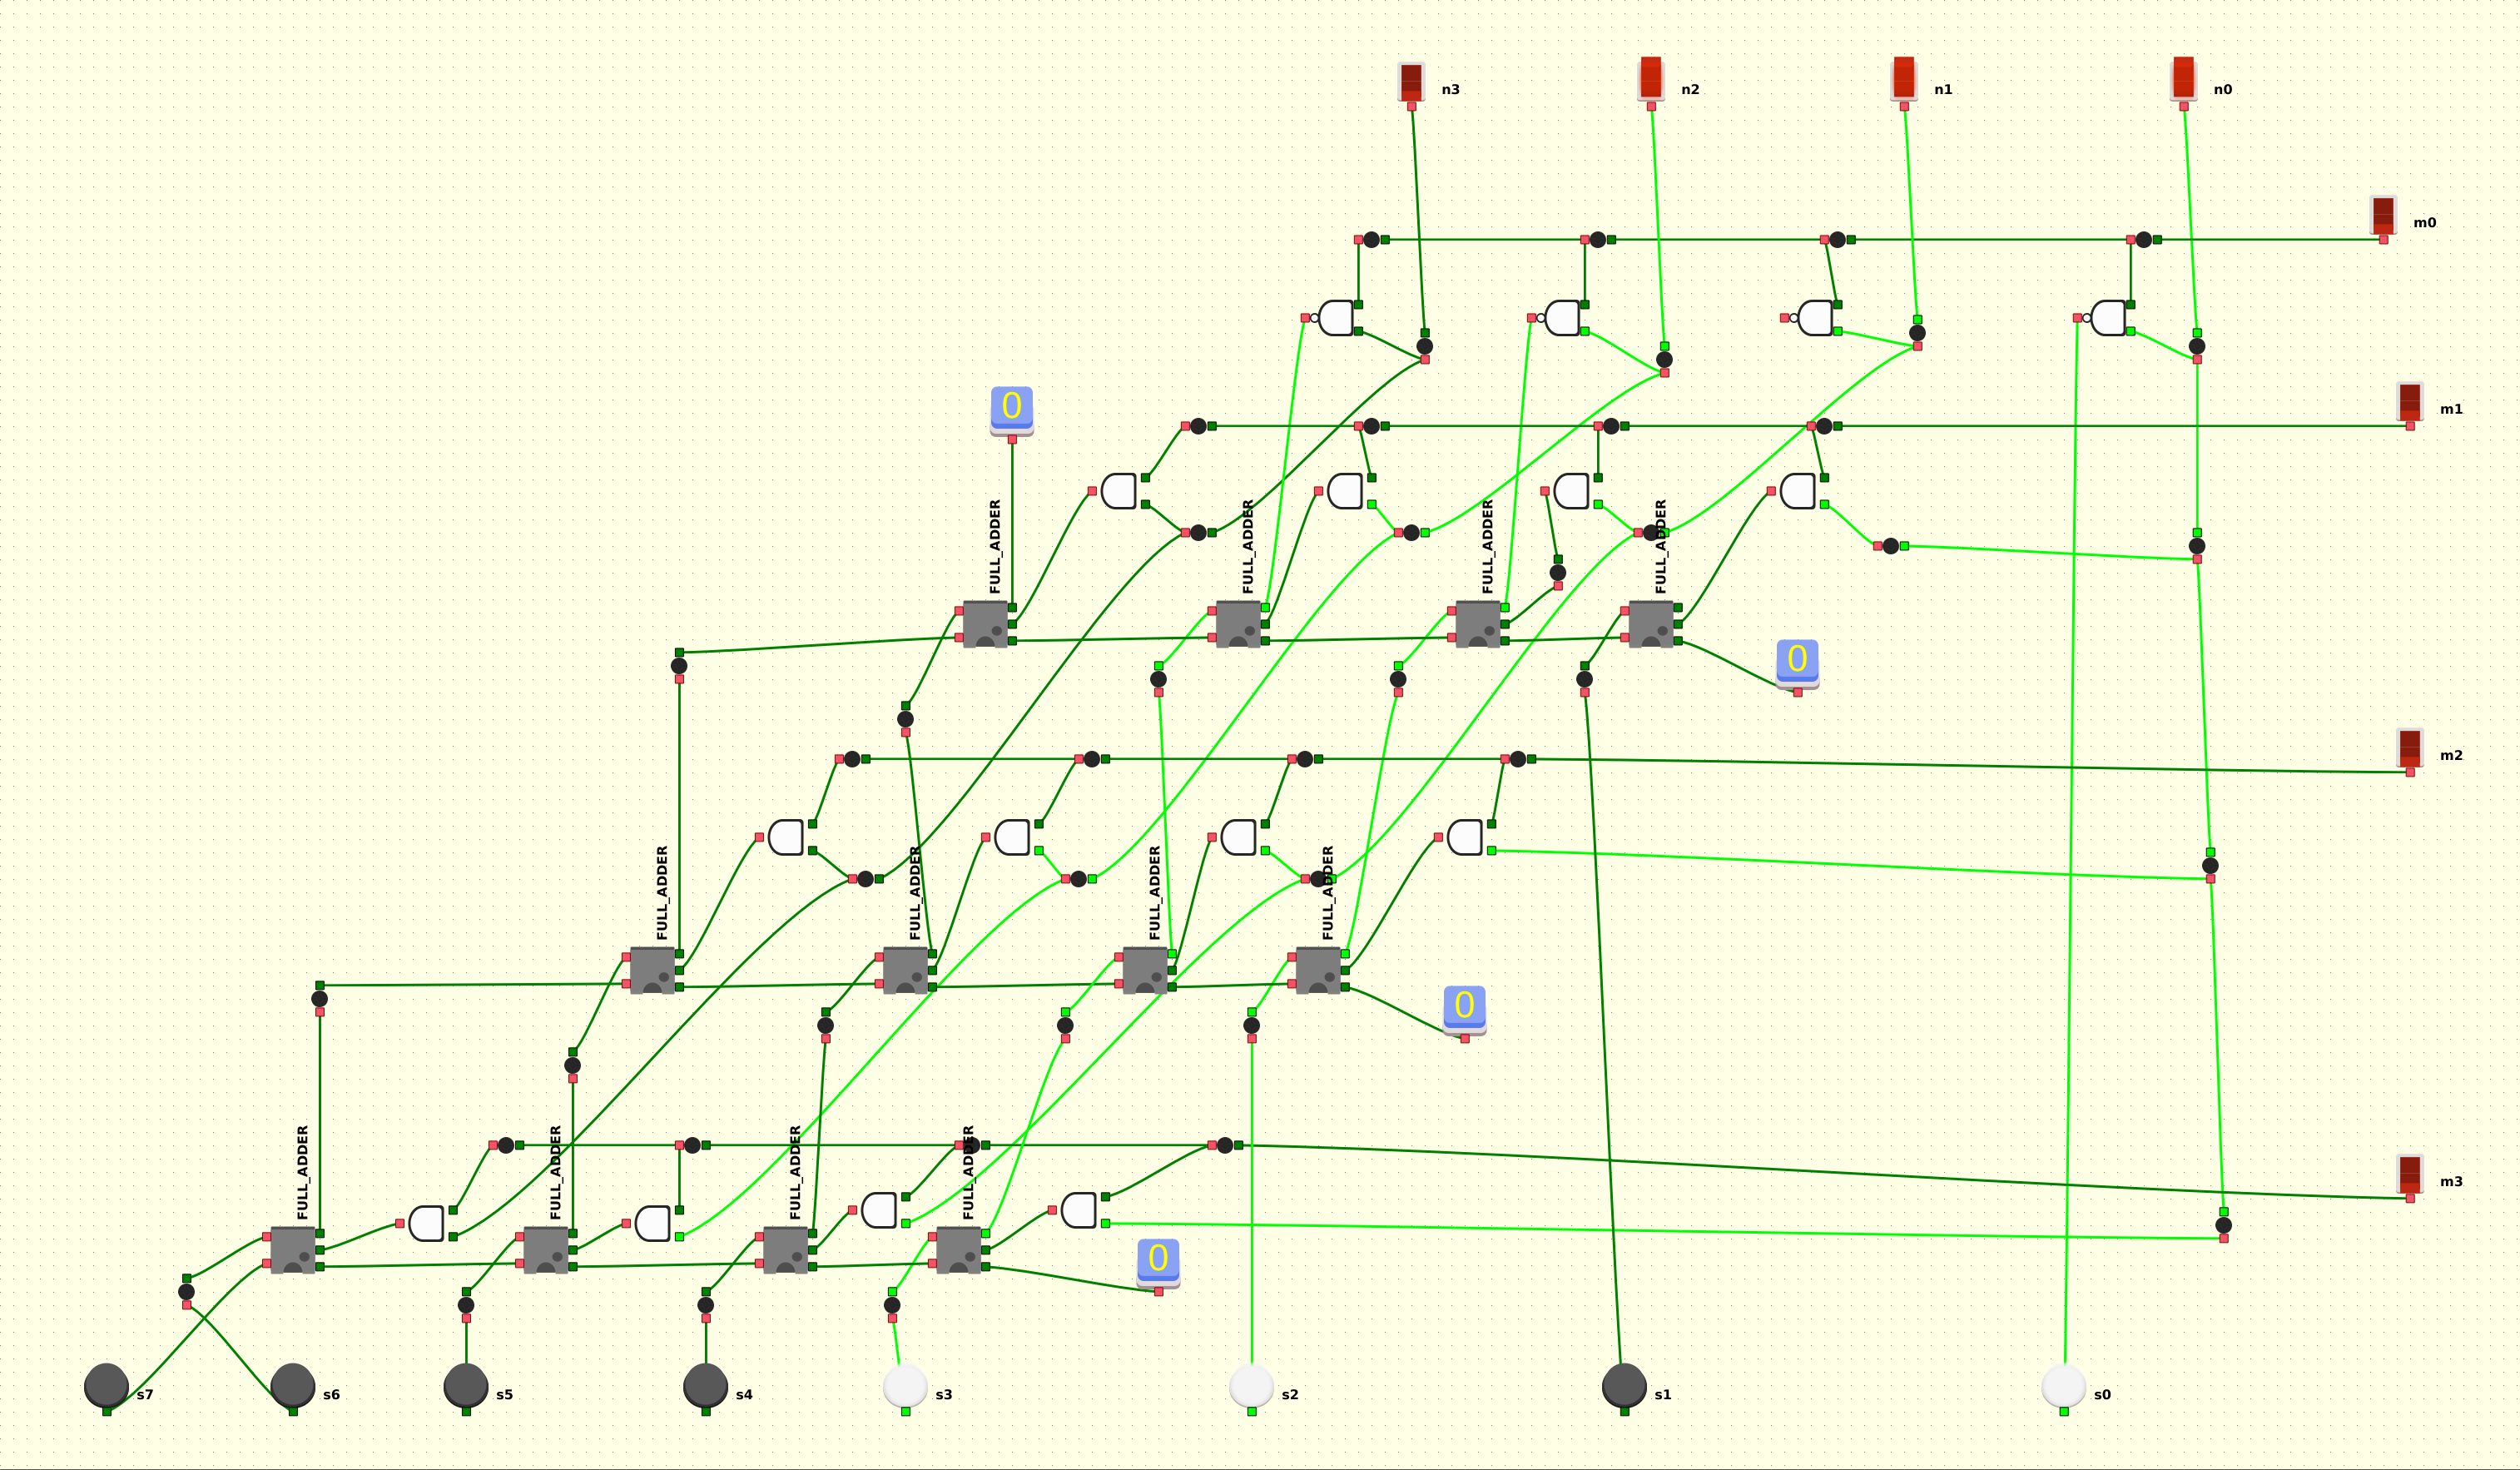
\includegraphics[width=15cm]{mult.png}
\caption{Multiplicador}
\label{fig:CL_logo}
\end{figure}

\section{A e soma/subtração do produto de C e D}

Para estes utilizei os circuitos disponibilizados do laboratório 03.

\section{Circuito completo}

Com a junção de todos estes resulta no seguinte circuito:
\\
\\
\\
\\
\\

\begin{figure}[!h]
\centering
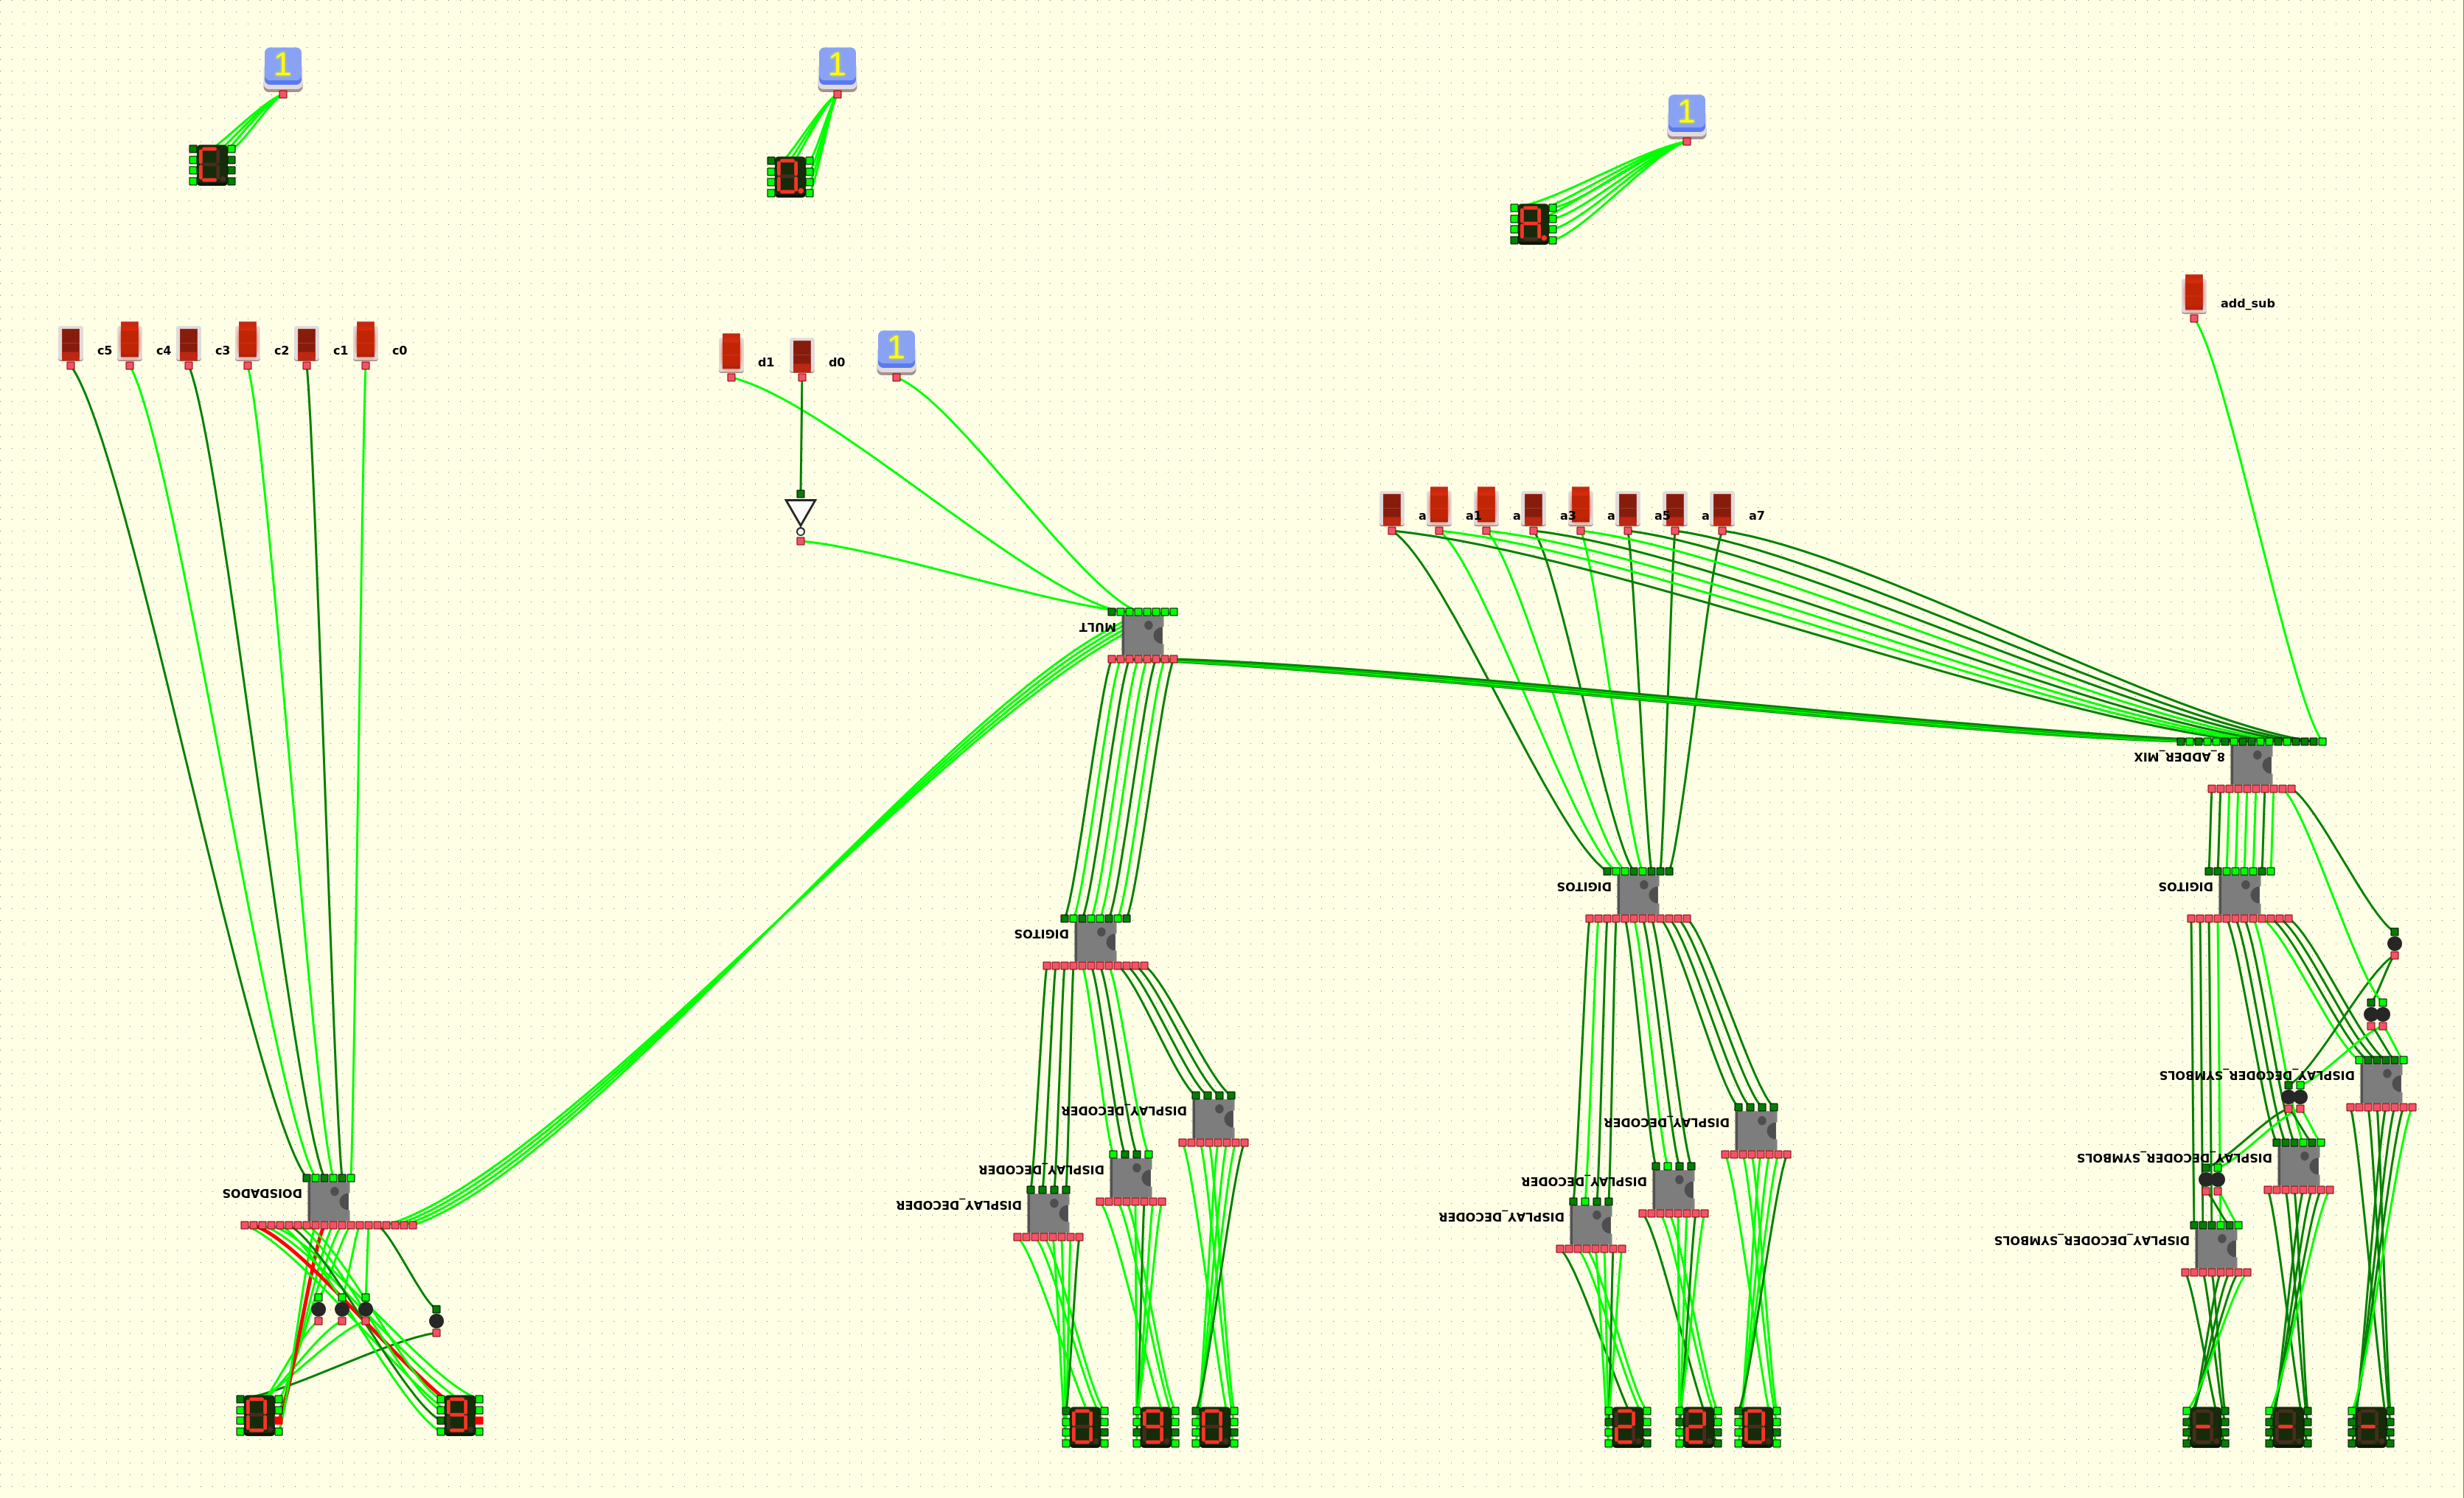
\includegraphics[width=15cm]{main.png}
\caption{Circuito final}
\label{fig:CL_logo}
\end{figure}

O arquivo .panda pode ser encontrado no seguinte \href{https://github.com/aamgoulart/circuitosDigitais}{repositório}

\end{document}
